%! TEX TS-program = xelatex
\documentclass[11pt, answers, addpoints]{exam}

% dfrac, therefore, etc.
\usepackage{amsmath, amsthm, amssymb}

% unitts
\usepackage{siunitx}

% diagrams and graphs
\usepackage{tikz}
\usepackage{pgfplots}
\pgfplotsset{compat=1.18}

% line spacing
\usepackage{setspace}

% cancellation
\usepackage{cancel}

% cases
\usepackage{cases}

% better labelling
\usepackage[nolabel, final]{showlabels}

% font
\usepackage[T1]{fontenc}
\usepackage[lf]{MinionPro}

\newcommand{\reals}{\mathbb{R}}
\newcommand{\ints}{\mathbb{Z}}
\newcommand{\posints}{\mathbb{Z}^{+}}
\newcommand{\rationals}{\mathbb{Q}}
\newcommand{\complexes}{\mathbb{C}}
\renewcommand{\frac}[2]{\dfrac{#1}{#2}}

\pagestyle{plain}

\begin{document}
\onehalfspacing%

\begin{center}
	\Large
	\textbf{SBGE Paper C (2022)}
\end{center}

\bracketedpoints%
\pointsinrightmargin%

\begin{questions}
	\question[2] A particular brand of hand sanitiser is in the shape
	of a cuboid as shown below:
	\begin{figure}[htpb]
		\centering
		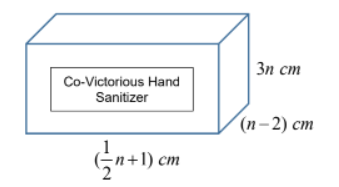
\includegraphics[scale=0.7]{./q1.png}
		\label{fig:sanitiser}
	\end{figure}

	Find and simplify an expression in terms of \(n\) for the volume of the
	hand sanitiser.

	\begin{solution}
		\begin{align*}
			\text{volume of hand sanitiser} & = 3n\left(\frac{1}{2}n + 1\right)(n - 2)                     \\
			                                & = \left(\frac{3}{2}n^{2} + 3n\right)(n - 2)                  \\
			                                & = \frac{3}{2}n^{3} + 3n^{2} - 3n^{2} - 6n                    \\
			                                & = \left(\frac{3}{2}n^{3} - 6n\right) \si{\centi\metre\cubed}
		\end{align*}
	\end{solution}


	\question Factorise completely:
	\begin{parts}
		\part[2] \(6x^{3} + 2x^{2}y - 4xy^{2}\)
		\begin{solution}
			\begin{align*}
				6x^{3} + 2x^{2}y - 4xy^{2} & = 2x\left(3x^{2} + xy - 2y^{2}\right) \\
				                           & = 2x(3x - 2y)(x + y)
			\end{align*}
		\end{solution}

		\part[3] \({(2x + 1)}^{2} - {\left(x^{2} + x + 1\right)}^{2}\)
		\begin{solution}
			\begin{align*}
				(2x + 1)^{2} - {\left(x^{2} + x + 1\right)}^{2} & = \left(2x + 1 + x^{2} + x + 1\right)\left(2x + 1 - x^{2} - x - 1\right) \\
				                                                & = \left(x^{2} + 3x + 2\right)\left(-x^{2} + x\right)                     \\
				                                                & = -x(x + 1)(x + 2)(x - 1)
			\end{align*}
		\end{solution}
	\end{parts}


	\question Simplify:
	\begin{parts}
		\part[3] \(\frac{3c}{1 - c} + \frac{3}{c - 1}\)
		\begin{solution}
			\begin{align*}
				\frac{3c}{1 - c} + \frac{3}{c - 1} & = \frac{3c - 3}{1 - c} \\
				                                   & = -3
			\end{align*}
		\end{solution}

		\part[3] \(\frac{a^{2} - b^{2}}{{(a - b)}^{2}} \div \frac{1}{a^{2} + b^{2}} \times \frac{1}{{(a - b)^{2} + 2ab}}\)
		\begin{solution}
			\begin{align*}
				 & \frac{a^{2} - b^{2}}{{(a - b)}^{2}} \div \frac{1}{a^{2} + b^{2}} \times \frac{1}{{(a - b)^{2} + 2ab}}                                   \\
				 & = \frac{(a + b)\cancel{(a - b)}}{(a - b)\cancel{(a - b)}} \cdot \frac{\cancel{a^{2} + b^{2}}}{1} \cdot \frac{1}{\cancel{a^{2} + b^{2}}} \\
				 & = \frac{a + b}{a - b}
			\end{align*}
		\end{solution}
	\end{parts}


	\question[3] Make \(h\) the subject of the formula: \(\sqrt{1 - hp} = p\).
	\begin{solution}
		\begin{align*}
			\sqrt{1 - hp} & = p                   \\
			1 - hp        & = p^{2}               \\
			hp            & = 1 - p^{2}           \\
			h             & = \frac{1 - p^{2}}{p} \\
		\end{align*}
	\end{solution}

	\question%
	\begin{parts}
		\part[3] Solve the equation: \(\frac{1}{x} + \frac{2}{3x} = \frac{3}{x + 1}\).
		\begin{solution}
			\begin{align*}
				\frac{1}{x} + \frac{2}{3x} & = \frac{3}{x + 1} \\
				\frac{5}{3x}               & = \frac{3}{x + 1} \\
				5(x + 1)                   & = 9x              \\
				4x                         & = 5               \\
				x                          & = \frac{5}{4}
			\end{align*}
		\end{solution}

		\part[1] Hence or otherwise, solve the equation \(\frac{1}{x + 1} + \frac{2}{3x + 3} = \frac{3}{x + 2}\).
		\begin{solution}
			\begin{align*}
				\frac{1}{x + 1} + \frac{2}{3x + 3}   & = \frac{3}{x + 2}       \\
				\frac{1}{x + 1} + \frac{2}{3(x + 1)} & = \frac{3}{(x + 1) + 1} \\
				\therefore x + 1                     & = \frac{5}{4}           \\
				\therefore x                         & = \frac{1}{4}           \\
			\end{align*}
		\end{solution}
	\end{parts}


	\question Given that \(a^{2} - 49 = 9951\),
	\begin{parts}
		\part[1] find the positive value of \(a\).
		\begin{solution}
			\begin{align*}
				a^{2} - 49 & = 9951             \\
				a          & = \sqrt{9951 + 49} \\
				           & = 100
			\end{align*}
		\end{solution}

		\part[3] Hence, find two factors of \(9951\) which are between \(50\) and \(200\).
		\begin{solution}
			\begin{align*}
				a^{2} - 49 & = 9951 \\
				(a+7)(a-7) & = 9951 \\
			\end{align*}
			When \(a = 100\), the two factors of \(9951\) are \(a + 7 = 107\) and \(a - 7 = 93\).
		\end{solution}
	\end{parts}


	\question[4] \underline{By defining two variables, solve the following problem using SLEs.}

	Two books, \textit{A} and \textit{B}, have a total of \(500\) pages. If the number of pages in Book \textit{A} is \(12\) less than \(3\) times the number of pages in Book \textit{B}, calculate the number of pages in each book.

	\begin{solution}
		Let the number of pages in Books \textit{A} and \textit{B} be \(a\) and \(b\) respectively.
		\begin{align}
			a + b & = 500\label{eq:71}     \\
			a     & = 3b - 12\label{eq:72}
		\end{align}
		Substitute \eqref{eq:72} into \eqref{eq:71}:
		\begin{align*}
			3b - 12 + b  & = 500 \\
			4b           & = 512 \\
			b            & = 128 \\
			\therefore a & = 372
		\end{align*}
		The number of pages in Books \textit{A} and \textit{B} is \(372\) and \(128\) respectively.
	\end{solution}


	\question An ice-cream maker machine can hold 60 \si{\litre} of ice-cream mix. It was discovered that
	\begin{parts}
		\part[1] when the temperature of the machine is set at \num{-10}\si{\celsius}, \(x\) \si{\litre} of ice-cream mix can be frozen per \si{\minute}.
		Write down an expression in terms of \(x\) for the time taken to freeze 60 \si{\litre} of ice cream mix at \num{-10}\si{\celsius} in \si{\minute}.
		\begin{solution}
			The time taken would be \(\frac{60}{x}\) \si{\minute}.
		\end{solution}

		\part[1] when the temperature of the machine was set at \num{-5}\si{\celsius}, \((x - 2)\) \si{\litre} of ice cream mix can be frozen per minute.
		Write down an expression in terms of \(x\) for the time taken to freeze 60 \si{\litre} of ice cream mix at \qty{-5}{\celsius} in \si{\minute}.
		\begin{solution}
			The time taken would be \(\frac{60}{x - 2}\) \si{\minute}.
		\end{solution}

		\part[2] it takes \qty{1.5}{\min} longer to freeze the ice cream mix at a higher temperature. Write down an equation in \(x\), and show that it simplifies to \(x^{2} - 2x - 80 = 0\).
		\begin{solution}
			\begin{align*}
				\frac{60}{x - 2} - \frac{60}{x} & = \frac{3}{2} \\
				\frac{120}{x(x - 2)}            & = \frac{3}{2} \\
				3x^{2} - 6x                     & = 240         \\
				x^{2} - 2x - 80                 & = 0           \\
			\end{align*}
		\end{solution}

		\part[2] \label{part:9d} Solve the equation \(x^{2} - 2x - 80 = 0\).
		\begin{solution}
			\begin{align*}
				x^{2} - 2x - 80                        & = 0  \\
				(x + 8)(x - 10)                        & = 0  \\
				\therefore x = -8 \text{ (rej.) or } x & = 10
			\end{align*}
		\end{solution}

		\part[1] Explain why you have to reject one of the solutions obtained in (\ref{part:9d}).
		\begin{solution}
			One of the solutions, \(x = -8\), is negative, which cannot represent the number of litres of ice cream frozen per \si{\min}.
		\end{solution}
	\end{parts}


	\question The diagram below shows the line \(L_{1}\), \(y = ax + b\).
	\begin{figure}[htpb]
		\centering
		\begin{tikzpicture}
			\begin{axis}[domain=-3:6, axis x line=middle, axis y line=middle, xlabel=\(x\), ylabel=\(y\), xtick={-2}, ytick={4}, xmin=-3, ymin=-3, xmax=3]
				\addplot[black, thick] {2 * x + 4};
			\end{axis}
		\end{tikzpicture}
	\end{figure}

	\begin{parts}
		\part[2] State the values of \(a\) and \(b\).
		\begin{solution}
			\(a = 2\), \(b = 4\).
		\end{solution}

		\part[2] Find the equation of another line, \(L_{2}\), which
		passes through the point \((5, 9)\) and is parallel to \(L_{1}\).
		\begin{solution}
			\begin{align*}
				y - y_{1} & = m(x - x_{1}) \\
				y - 9     & = 2(x - 5)     \\
				y         & = 2x - 1       \\
			\end{align*}
		\end{solution}

		\part[1] Does the point \((3, 10)\) lie on line \(L_{2}\)? Explain.
		\begin{solution}
			The point \((3, 10)\) does not lie on \(L_{2}\). Substituting the values of \(x = 3\) and \(y = 10\) into the equation \(y = 2x - 1\) makes the equation false.
		\end{solution}
	\end{parts}
\end{questions}
\end{document}
